\documentclass[8pt, a4paper, oneside, twocolumn]{extarticle}
\usepackage{graphicx}
\usepackage[export]{adjustbox}
\usepackage[compact]{titlesec}  % documentation: http://mirror.iopb.res.in/tex-archive/macros/latex/contrib/titlesec/titlesec.pdf  
\usepackage{kotex}
\usepackage[left=0.8cm, right=0.8cm, top=2cm, bottom=0.3cm, a4paper]{geometry}
\usepackage{amsmath}
\usepackage{ulem}
\usepackage{amssymb}
\usepackage{minted}  % syntax highlighting
\usepackage{xcolor}
\usepackage{enumitem}
\setlist{nolistsep}
\usepackage{fancyhdr} % documentation: http://ctan.math.utah.edu/ctan/tex-archive/macros/latex/contrib/fancyhdr/fancyhdr.pdf
\usepackage{lastpage}  % just so that we can use \pageref {LastPage}
\usepackage{color, hyperref}
% The lines in the table of contents become links to the corresponding pages in the document by simply adding in the preamble of the document the line
\usepackage{tikz}
\usetikzlibrary{positioning,chains,fit,shapes,calc}
\newcommand{\bck}{
    \textbackslash
}
\newcommand{\iph}[2]{
    \includegraphics[width=#1\textwidth,height=#1\textheight,keepaspectratio]{#2}
}
\newcommand{\ph}[1]{
    \includegraphics[width=0.5\textwidth,height=0.5\textheight,keepaspectratio]{#1}
}
\newcommand{\ita}[1]{
    \textit{#1}
}
\newcommand{\swastik}[1]{%
    \begin{tikzpicture}[#1]
        \draw (-1,1)  -- (-1,0) -- (1,0) -- (1,-1);
        \draw (-1,-1) -- (0,-1) -- (0,1) -- (1,1);
    \end{tikzpicture}%
}
\titlespacing*{\section}
{0pt}{0px plus 1px minus 0px}{-2px plus 0px minus 0px}
\titlespacing*{\subsection}
{0pt}{0px plus 1px minus 0px}{0px plus 3px minus 3px}
\titlespacing*{\subsubsection}
{0pt}{0px plus 1px minus 0px}{0px plus 3px minus 3px}
\setlength{\columnseprule}{0.4pt}
\DeclareRobustCommand{\stirling}{\genfrac\{\}{0pt}{}}
\setlength{\parindent}{0pt}  % so that there is no indent of paras.
\setminted{breaklines=true, tabsize=2, breaksymbolleft=}
\begin{document}
\title{\swastik {scale = 0.2} {}Compiler Short Revision Notes{} \swastik {scale = 0.2}}
\author{Sourabh Aggarwal}
\date{Compiled on \today}
\maketitle
\pagenumbering{roman}
\tableofcontents
\newpage
\thispagestyle{fancy}  % else it was not giving fancy header to the first page
\pagenumbering{arabic}
\section{Intro And ML Lex}

\textcolor{red}{some part is in class notes}

$(a \odot b) \vert \epsilon$ represents the language \{"", "ab"\}. 
In writing regular expressions, we will sometimes omit the concatenation 
symbol or the epsilon, and we will assume that Kleene closure "binds tighter" 
than concatenation, and concatenation binds tighter than alternation; so that 
$ab \vert c$ means $(a \odot b) \vert c$, and $(a \vert)$ means $(a \vert \epsilon)$. 
Let us introduce some more abbreviations: [abed] means 
$(a \vert b \vert c \vert 
d)$, [b-g] means [bcdefg], [b-gM-Qkr] means [bcdefgMNOPQkr], M? 
means ($M \vert \epsilon$), and $M^+$ means ($M \odot M^*$). 

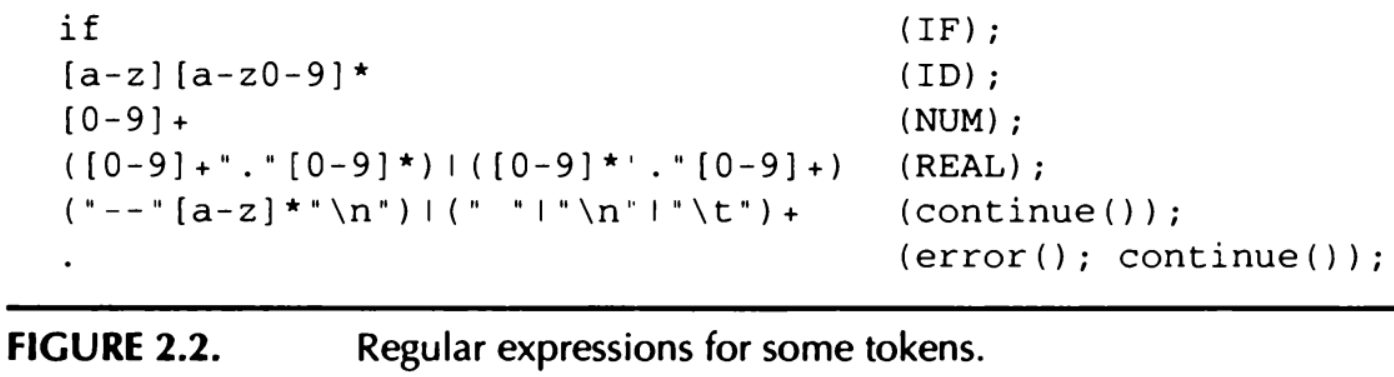
\includegraphics[width=0.5\textwidth,height=0.5\textheight,keepaspectratio]{reg}

Longest match: The longest initial substring of the input that can match any 
regular expression is taken as the next token. 

Rule priority: For a \textbf{particular} longest initial substring, the first regular  
expression that can match determines its token type. This means that the order of 
writing down the regular-expression rules has significance. 

So according to the rules, if8 match as a single 
identifier and not as the two tokens if and 8. And "if 89" begin with a 
reserved word and not by an identifier by rule priority rule. 


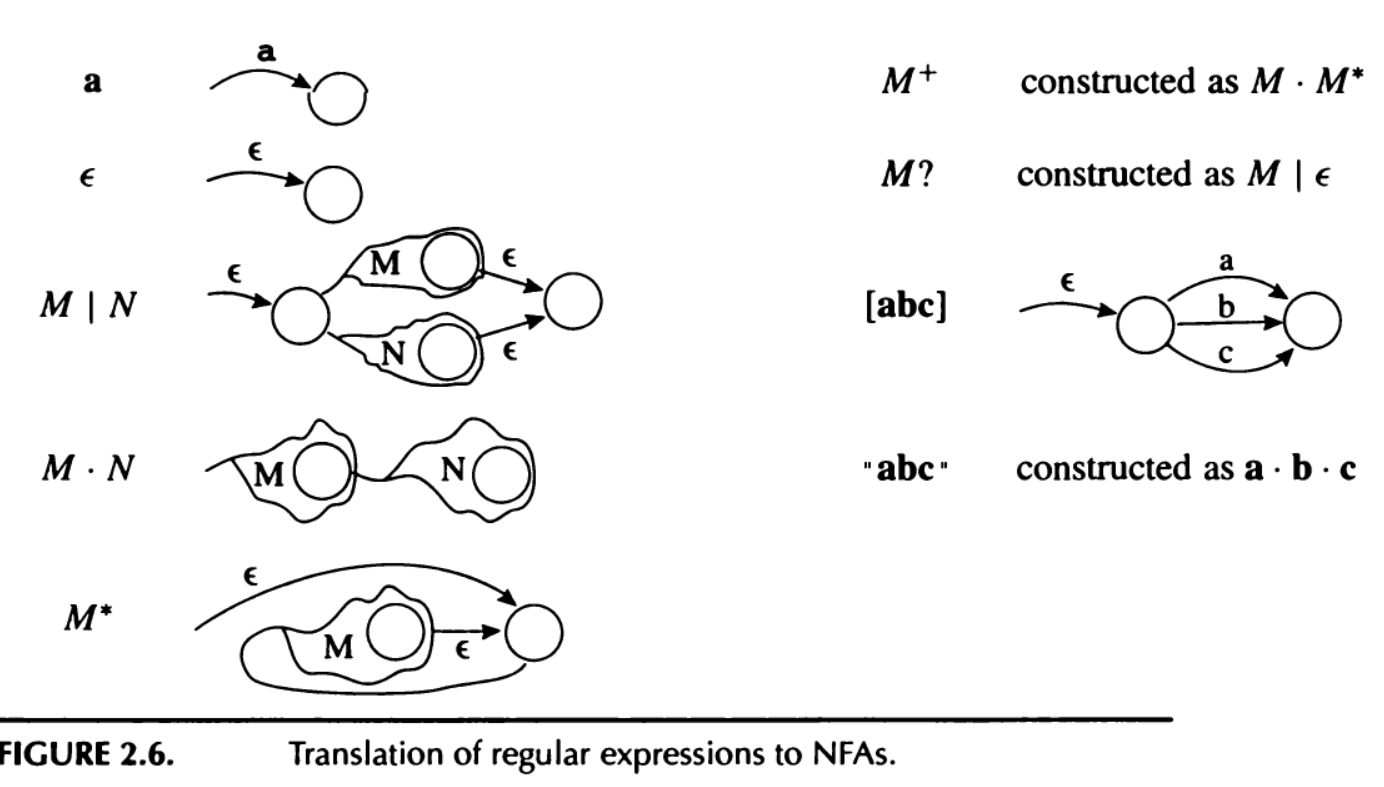
\includegraphics[width=0.5\textwidth,height=0.5\textheight,keepaspectratio]{rtnfa}


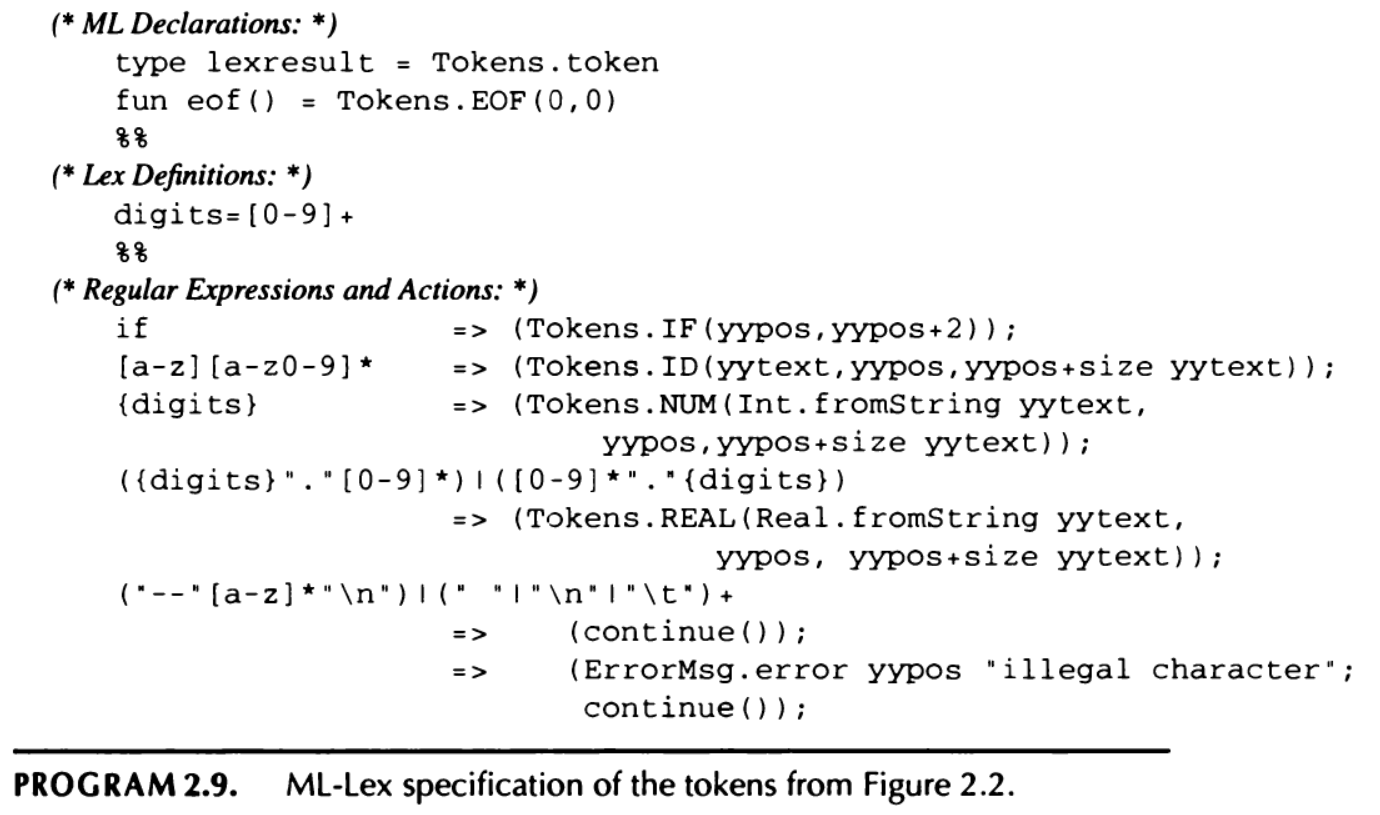
\includegraphics[width=0.5\textwidth,height=0.5\textheight,keepaspectratio]{lex}


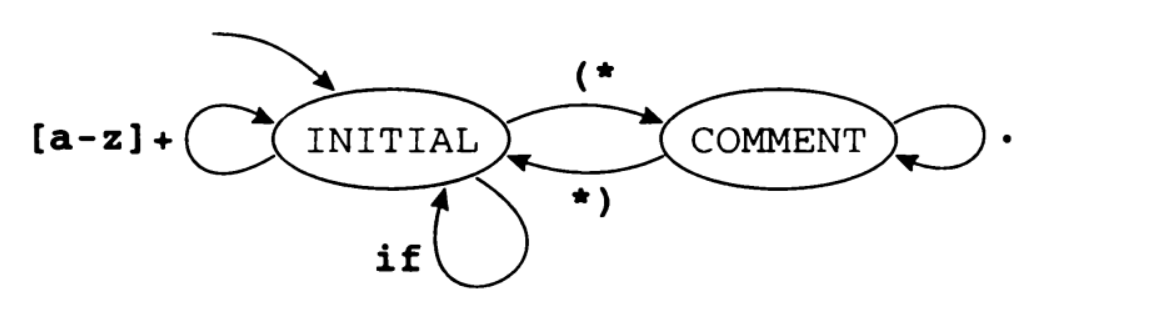
\includegraphics[width=0.5\textwidth,height=0.5\textheight,keepaspectratio]{lex3}

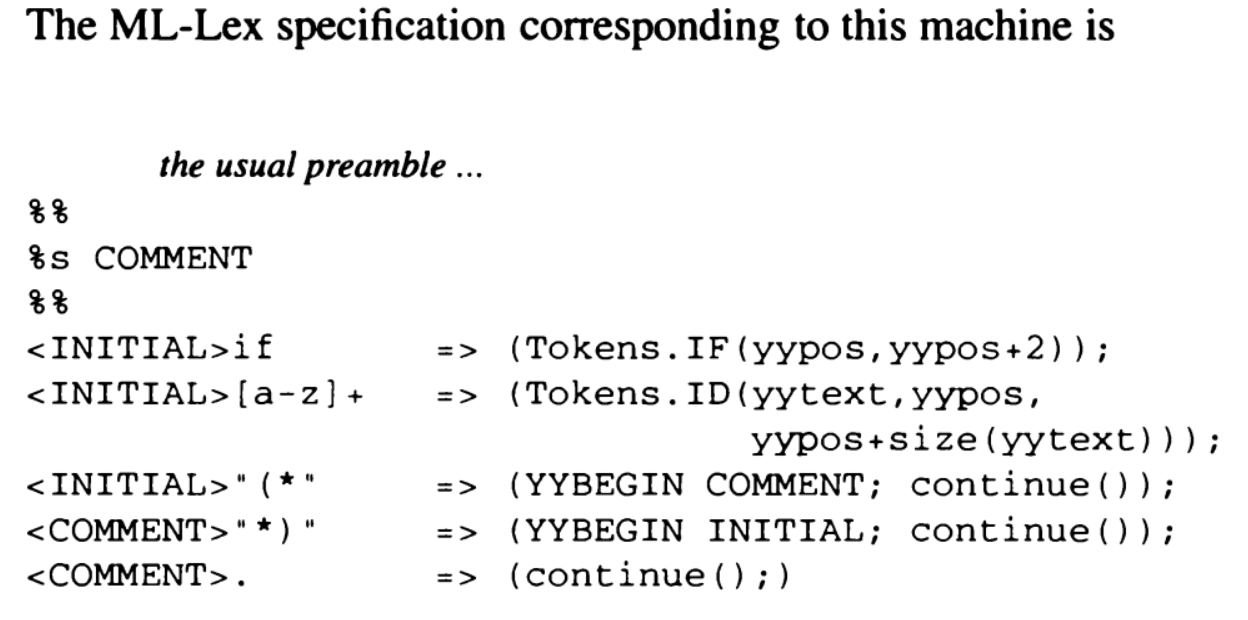
\includegraphics[width=0.5\textwidth,height=0.5\textheight,keepaspectratio]{lex4}


Certain rules
\begin{itemize}
    \item     An individual character stands for itself, except for the reserved characters 
    \begin{minted}{cpp}
     ? * + | ( ) ^ $ / ; . = < > [ { " \  $

    \end{minted}

    \item A backslash followed by one of the reserved characters stands for that character. 

    \item Inside the brackets, only the symbols \begin{minted}{cpp} 
    \ - ^ 
\end{minted}
 are reserved. An initial up-arrow \^{} stands for the complement of the characters listed, e.g. [\^{}abc] stands any character except a, b, or c.
    \item  To include \^{} literally in a bracketed set, put it anywhere but first; to include - literally in a set, put it first or last. 
    \item The dot . character stands for any character except newline, i.e. the same as \begin{minted}{cpp}
        [^\n]
    \end{minted}
    \item The following special escape sequences are available, inside or outside of square brackets: 
    \begin{minted}{SML}
    \b backspace
    \n newline
    \t horizontal tab
    \ddd where ddd is a 3 digit decimal escape
    \end{minted}
    \item Any regular expression may be enclosed in parentheses ( ) for syntactic (but, as
    usual, not semantic) effect
    \item A sequence of characters will stand for itself (reserved characters will be taken literally) if it is enclosed in double quotes " ".
    \item A postfix repetition range \{a, b\} where a and b are small integers stands for any number of repetitions between a and b of the preceding expression. The notation \{a\} stands for exactly a repetitions. Ex: [0-9]\{3\}
    Any three-digit decimal number. 
    \item The rules should match all possible input. If some input occurs that does not match any rule, the lexer created by ML-Lex will raise an exception LexError.
    \item  The user may recursively call the lexing function with lex(). (If \%arg is used, the lexing function may be re-invoked with the same argument by using continue().) This is convenient for ignoring white space or comments silently:
    \begin{minted}{SML}
    [\ \t\n]+       => ( lex());
    \end{minted}
    \item To switch start states, the user may call YYBEGIN with the name of a start state. 
\end{itemize}
\section{Parsing}

\textcolor{red}{some part is in class notes}

The parser returns an abstract syntax tree of the expression being evaluated. The parser gets tokens from the scanner to parse the input and build the AST. When an AST is
returned by the parser, the compiler calls the code generator to evaluate the tree and produce the target code.

There are two main parts to a compiler, the front end and back end. The front end
reads the tokens and builds an AST of a program. The back end generates the code
given the AST representation of the program. As presented in earlier chapters, the
front end consists of the scanner and the parser.

As before, we say that a language is a set of strings; each string is a finite
sequence of symbols taken from a finite alphabet. For parsing, the strings are
source programs, the symbols are lexical tokens, and the alphabet is the set
of token types returned by the lexical analyzer.

A leftmost
derivation is one in which the leftmost nonterminal symbol is always the one
expanded; in a rightmost derivation, the rightmost nonterminal is always next
to be expanded.

A parse tree is made by connecting each symbol in a derivation to the one
from which it was derived, as shown in Figure 3.3. Two different derivations
can have the same parse tree.

A grammar is ambiguous if it can derive a sentence with two different parse
trees.

Parsers must read not only terminal symbols such as +, -, num, and so on, but
also the end-of-file marker. We will use \$ to represent end of file.

Suppose S is the start symbol of a grammar. To indicate that \$ must come
after a complete S-phrase, we augment the grammar with a new start symbol
S' and a new production S' $\rightarrow$ S\$.

\textbf{Predictive Parsing:} Some grammars are easy to parse using a simple algorithm known as 
recursive descent. Predictive parsing works only on grammars where
the first terminal symbol of each subexpression provides enough information
to choose which production to use.

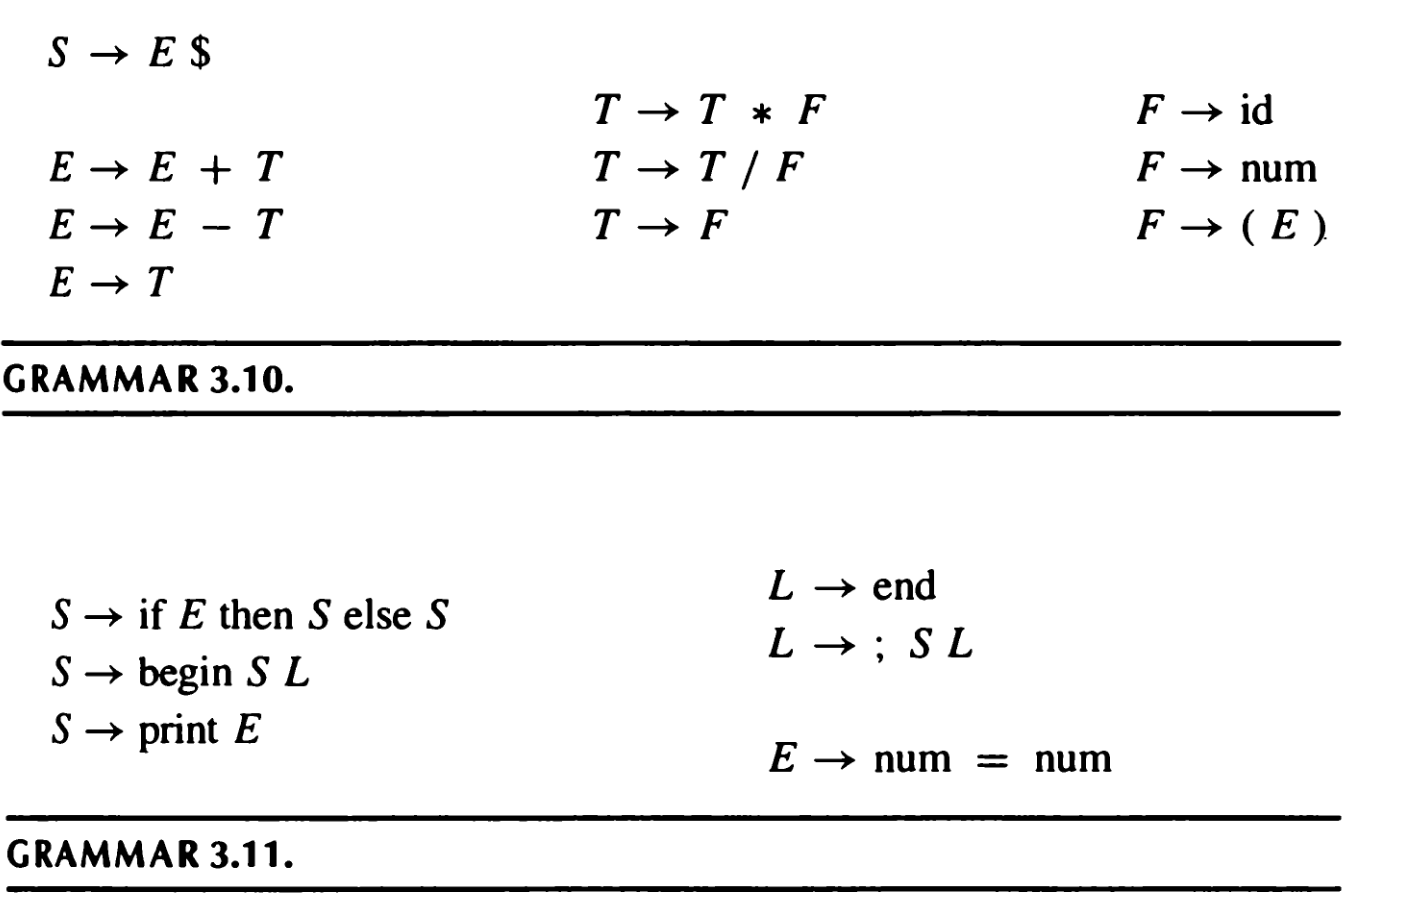
\includegraphics[width=0.5\textwidth,height=0.5\textheight,keepaspectratio]{pp}

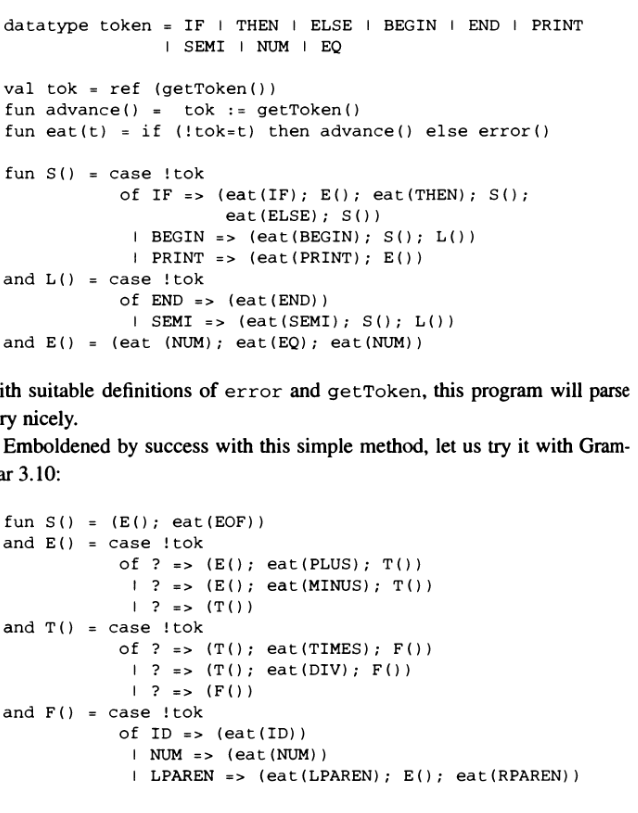
\includegraphics[width=0.5\textwidth,height=0.5\textheight,keepaspectratio]{pp2}

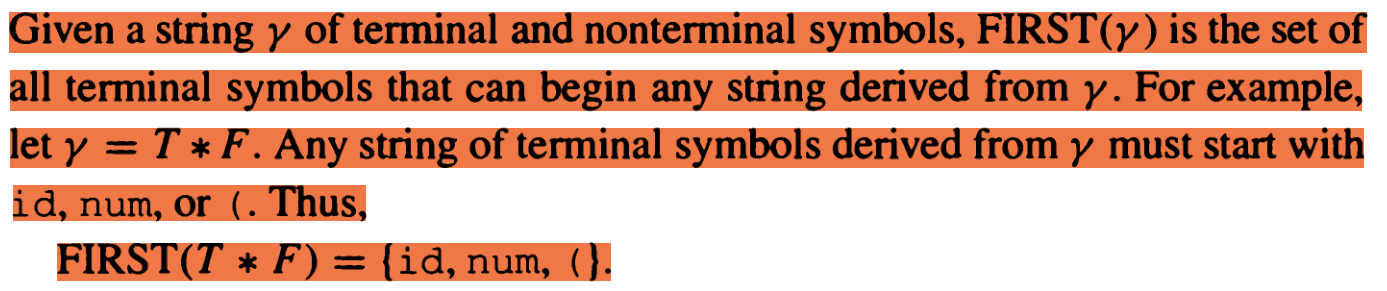
\includegraphics[width=0.5\textwidth,height=0.5\textheight,keepaspectratio]{first}

If two different productions $X \rightarrow \gamma_1 and X \rightarrow \gamma_2$ have the same left-
hand-side symbol $(X)$ and their right-hand sides have overlapping FIRST
sets, then the grammar cannot be parsed using predictive parsing.

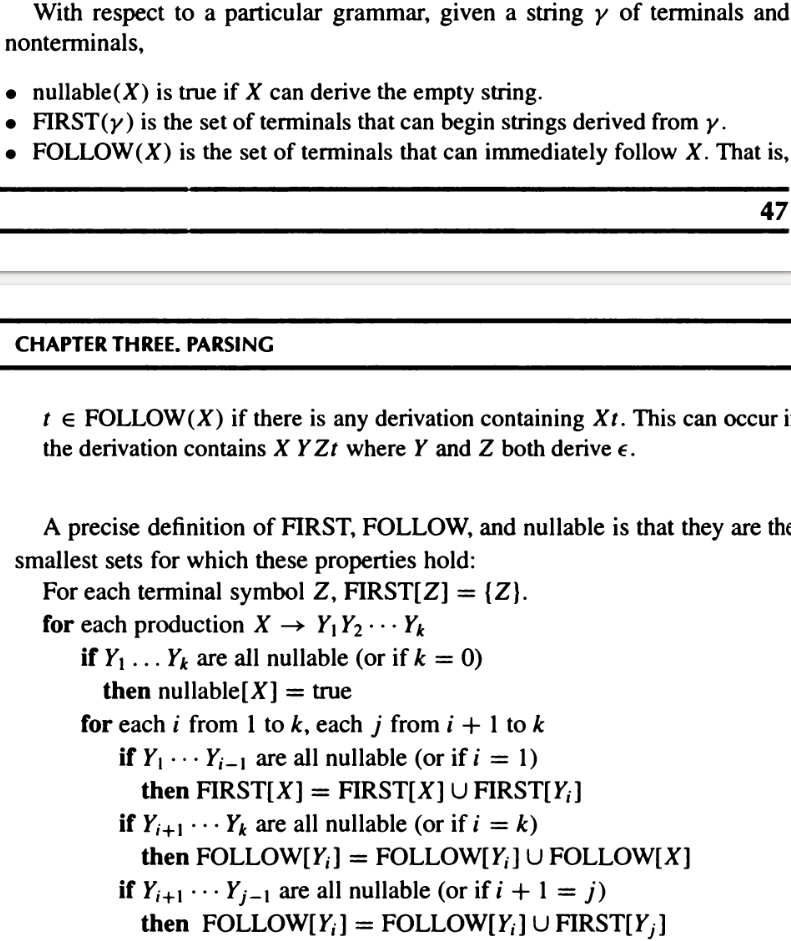
\includegraphics[width=0.5\textwidth,height=0.5\textheight,keepaspectratio]{follow}

\textbf{Error recovery in predictive parsing (LL (1)):}

\iph{0.5}{erpp}

\subsection{LR(0)}

\iph{0.5}{lr0}

Note: 'X' in Goto can be either a terminal or non terminal
 
Grammar is same as that written in notebook.

Shift (n): Advance input one token; push n on stack.

Reduced (k): Pop stack as many times as the number of
symbols on the right-hand side of rule k.
Let X be the left-hand-side symbol of rule k;
In the state now on top of stack, look up X to get "goto n";
Push n on top of stack.
\iph{0.5}{lr0g}

\iph{0.5}{lr01}

\iph{0.5}{lr02}



\subsection{SLR}

\iph{0.35}{slr}

\iph{0.5}{slr2}

\iph{0.5}{slrg1}

\iph{0.5}{slrg2}

\subsection{LR(1)}

\ph{lr1}

\ph{lr2}

\ph{hier}

\ph{yaccpref}

\ph{yaccpref2}

\ph{yaccpref3}

\ph{yaccpref4}

\ph{yaccpref5}

Popping states from the stack can lead to seemingly "im

\ph{err}

\ph{gerr}

\section{CH 5 (Not in syllabus) Semantic Analysis}
This phase is characterized by the maintenance of symbol tables (also called
environments) mapping identifiers to their types and locations.

\ph{sem1}

\ph{sem2}

\section{CH 6 Activation Records}
For the remainder of this chapter we will consider languages with stackable
local variables and postpone discussion of higher-order functions to 
Chapter 15.

\ph{r1}

\ph{r2}

\ph{r3}

\ph{r4}

\ph{r5}

\ph{r6}

\ph{r7}

\ph{r8}

Figure 6.2 shows a typical stack frame layout. The frame has a set of 
incoming arguments (technically these are part of the previous frame but they
are at a known offset from the frame pointer) passed by the caller. The 
return address is created by the CALL instruction and tells where (within the
calling function) control should return upon completion of the current 
function. Some local variables are in this frame; other local variables are kept in
machine registers. Sometimes a local variable kept in a register needs to be
saved into the frame to make room for other uses of the register; there is an
area in the frame for this purpose. Finally, when the current function calls
other functions, it can use the outgoing argument space to pass parameters.

Suppose a function g(...) calls the function f($a_1, \dots , a_n$). We say g is the
caller and f is the callee.
On entry to f, the stack pointer points to the first
argument that g passes to f. On entry, f allocates a frame by simply 
subtracting the frame size from the stack pointer SP. The old SP becomes the current frame pointer FP.

FP is a
"fictional" register whose value is always SP+framesize.
Why talk about a frame pointer at all? Why not just refer to all variables,
parameters, etc. by their offset from SP, if the frame size is constant? The
frame size is not known until quite late in the compilation process, when the
number of memory-resident temporaries and saved registers is determined.

Suppose a function f is using register r to hold a local variable and calls procedure g, which also uses r for
its own calculations. Then r must be saved (stored into a stack frame) before
g uses it and restored (fetched back from the frame) after g is finished using
it. But is it f's responsibility to save and restore the register, or g's? We say
that r is a caller-save register if the caller (in this case, f) must save and 
restore the register, and r is callee-save if it is the responsibility of the callee
(in this case, g).

therefore the
first k arguments (for k = 4 or k = 6, typically) of a function are passed in
registers $r_p, \dots, r_{p+k - 1}$ and the rest of the arguments are passed in memory.

\ph{r9}

\ph{r10}

\ph{r11}

To resolve the contradiction that
parameters are passed in registers, but have addresses too, the first k 
parameters are passed in registers; but any parameter whose address is taken must
be written to a memory location on entry to the function. To satisfy printf,
the memory locations into which register arguments are written must all be
consecutive with the memory locations in which arguments k + 1, k + 2, etc.
are written. Therefore, C programs can't have some of the arguments saved
in one place and some saved in another - they must all be saved contiguously.

When function g calls function f, eventually f must return. It needs to know
where to go back to. If the call instruction within g is at address a, then
(usually) the right place to return to is a + 1, the next instruction in g. This is
called the return address.

On modern machines, the call instruction merely puts the return address
(the address of the instruction after the call) in a designated register. A non-
leaf procedure will then have to write it to the stack (unless interprocedural
register allocation is used), but a leaf procedure will not.

Many of the local variables will be allocated to registers, as will the
intermediate results of expression evaluation. Values are written to memory
(in the stack frame) only when necessary for one of these reasons:

\ph{r12}

We will say that a variable escapes if it is passed by reference, its address
is taken (using C's \& operator), or it is accessed from a nested function.

Unfortunately, the conditions in our list don't manifest
themselves early enough. When the compiler first encounters the declaration
of a variable, it doesn't yet know whether the variable will ever be passed
by reference, accessed in a nested procedure, or have its address taken; and
doesn't know how many registers the calculation of expressions will require
An industrial-strength compiler must assign provisional locations
to all formals and locals, and decide later which of them should really go in registers.

In languages that allow nested function declarations, the inner functions may use variables declared in outer functions. This
language feature is called block structure.

There are several methods to allow inner functions to access outer ones:

\ph{r13}

I will describe in detail only the method of static links.

\ph{arpb}

\ph{r14}

\ph{r15}


\section{CH 7 Translation To Intermediate Code}
The front end of the compiler does lexical analysis, parsing,
semantic analysis, and translation to intermediate representation. The back
end does optimization of the intermediate representation and translation to
machine language.

\ph{ir1}

For our compiler the intermediate representation tree language is defined by the signature tree, as shown in figure

\ph{ir2}

Meaning:

expressions (exp), which stand for the computation of some value (possibly
with side effects):

\ph{ir3}

\ph{ir4}

\ph{ir5}

What should the representation of an abstract syntax expression Absyn.exp
be in the Tree language? At first it seems obvious that it should be Tree.exp.
However, this is true only for certain kinds of expressions, the ones that 
compute a value. Expressions that return no value (such as some procedure calls,
or while expressions in the Tiger language) are more naturally represented
by Tree.stm. And expressions with Boolean values, such as $a > b$, might
best be represented as a conditional jump - a combination of Tree.stm and
a pair of destinations represented by Temp. labels.
Therefore, we will make a datatype exp in the Translate module to
model these three kinds of expressions:

\ph{ir6}

Sometimes we will have an expression of one kind and we will need to
convert it to an equivalent expression of another kind. For example, the Tiger
statement

flag := $(a>b \vert c<d)$

\ph{ir7}

\ph{ir8}

\ph{ir9}

\section{CH 8 Basic Blocks And Traces}
It's useful to be able to evaluate the subexpressions of an 
expression in any order. If tree expressions did not contain ESEQ and CALL nodes,
then the order of evaluation would not matter.

\ph{81}

We can take any tree and rewrite it into an equivalent tree without any of
the cases listed above. Without these cases, the only possible parent of a SEQ
node is another SEQ; all the SEQ nodes will be clustered at the top of the tree.
This makes the SEQs entirely uninteresting; we might as well get rid of them
and make a linear list of Tree.stms.

The transformation is done in three stages: First, a tree is rewritten into a
list of canonical trees without SEQ or ESEQ nodes; then this list is grouped
into a set of basic blocks, which contain no internal jumps or labels; then
the basic blocks are ordered into a set of traces in which every CJUMP is
immediately followed by its false label.

\ph{82}

How can the ESEQ nodes be eliminated? The idea is to lift them higher and
higher in the tree, until they can become SEQ nodes.

\ph{83}

\ph{84}

\ph{85}

\ph{86}

\ph{87}

\ph{88}

\ph{89}

\ph{811}

\ph{812}

\ph{813}

\ph{814}

\ph{815}

\ph{816}

We will apply this algorithm to each function-body in turn. The procedure
"epilogue" (which pops the stack and returns to the caller) will not be part of
this body, but is intended to follow the last statement. When the flow of 
program execution reaches the end of the last block, the epilogue should follow.
But it is inconvenient to have a "special" block that must come last and that
has no JUMP at the end. Thus, we will invent a new label done - intended
to mean the beginning of the epilogue - and put a JUMP(NAME done) at the
end of the last block.

Now the basic blocks can be arranged in any order, and the result of executing
the program will be the same - every block ends with a jump to the 
appropriate place. We can take advantage of this to choose an ordering of the blocks
satisfying the condition that each CJUMP is followed by its false label.

At the same time, we can also arrange that many of the unconditional
jumps are immediately followed by their target label. This will allow the
deletion of these jumps, which will make the compiled program run a bit
faster.

\ph{818}

\ph{819}

\ph{820}

\section{CH 9 Instruction Selection}

Highlighting done in pdf.

\section{CH 10 Liveness Analysis}

Highlighting done in pdf.

\section{CH 11 Register Allocation}

\textcolor{red}{Everything in class notes}

\section{CH 13 Garbage Collection}

\textcolor{red}{Everything in class notes}

\end{document}
